\documentclass[aps,prd,twocolumn,superscriptaddress,nofootinbib,longbibliography,floatfix,showkeys,amsmath,amssymb,10pt]{revtex4-2}

\usepackage{mathptmx}
\usepackage{amsthm}
\usepackage{graphicx}
\usepackage{booktabs}
\usepackage{xcolor}
\usepackage{enumitem}
\usepackage[colorlinks=true,linkcolor=blue!50!black,citecolor=blue!50!black,urlcolor=blue!50!black,bookmarksnumbered=true]{hyperref}
\usepackage{orcidlink}
\usepackage{microtype}
\usepackage{xurl}

\makeatletter
\AtBeginDocument{\def\NAT@bibsetup{\setlength{\labelwidth}{\z@}%
 \setlength{\labelsep}{0.5em}\setlength{\itemindent}{\z@}%
 \setlength{\listparindent}{\z@}\setlength{\topsep}{\z@}%
 \setlength{\parsep}{\z@}\NATx@bibsetup}}
\let\write@bibliographystyle\relax
\let\bibliography@latex\@gobble
\makeatother

\tolerance=2000
\emergencystretch=2em
\hbadness=2000
\hfuzz=1pt
\raggedbottom

\newtheorem{theorem}{Theorem}
\newtheorem{lemma}[theorem]{Lemma}
\newtheorem{proposition}[theorem]{Proposition}
\newtheorem{corollary}[theorem]{Corollary}
\theoremstyle{definition}
\newtheorem{definition}[theorem]{Definition}
\theoremstyle{remark}
\newtheorem{remark}[theorem]{Remark}

\newcommand{\Z}{\mathbb{Z}}
\newcommand{\LRC}{\mathrm{LRC}}
\newcommand{\figw}{\columnwidth}
\newenvironment{wtable}{\begin{table*}[t]}{\end{table*}}
\def\zenodoID{}% version DOI of the Zenodo archive; empty until it is minted
\newcommand{\archivelink}{\ifx\zenodoID\empty\url{https://github.com/creelie/Math-repo1}%
 \else\href{https://doi.org/\zenodoID}{doi:\zenodoID}\fi}

\setlength{\emergencystretch}{3em}
\hyphenation{Sung-ka-wi-chai Tra-kul-thong-chai Al-li-kve-re}

\begin{document}

\title{Prime Divisibility for Sixteen Lonely Runners}

\author{Deep Bhattacharjee\,\orcidlink{0000-0003-0466-750X}}
\email{itsdeep@live.com}
\thanks{$*$\,Corresponding author. Second address:
\nolinkurl{d.bhattacharjee@erl-forschung.de}.}
\affiliation{Formerly, Electro-Gravitational Space Propulsion Laboratory
(EGSPL), Bhubaneswar, Odisha 751030, India}
\affiliation{Formerly, University of Calcutta, Senate House, 87/1 College
Street, Kolkata 700073, West Bengal, India}

\author{Ushashi Bhattacharya\,\orcidlink{0009-0002-2254-3914}}
\email{rai.bhattacharya.in@gmail.com}
\affiliation{Formerly, National Taiwan University, Taipei 106319, Taiwan}

\date{20 October 2026}

\begin{abstract}
\itshape
We prove that the speeds of any counterexample to the lonely runner conjecture for sixteen runners with no common factor have a product below an explicit bound and divisible by 720720 and by each of the primes 23, 29, 31, 179, 239, 269, 271, 281 and 283. The conjecture for sixteen runners therefore follows from a finite list of prime checks of the same kind. Two tools carry the method of the fifteen-runner case one step further: a shift lemma for powers of two, and binary lifting to greater depth.
\par\medskip\upshape\noindent
\textit{2020 Mathematics Subject Classification.} Primary 11J71;
Secondary 11H06, 52C07, 68V05.
\end{abstract}

\keywords{lonely runner conjecture; view obstruction; lattice flag bound;
computer-assisted proof}

\maketitle

\makeatletter
\renewcommand\l@subsection[2]{}
\renewcommand\l@subsubsection[2]{}
\makeatother
\tableofcontents

\section{Introduction}\label{sec:intro}

For a real number $x$ let $\|x\|$ be its distance to the nearest integer.
The Lonely Runner Conjecture $\LRC(k)$ asserts that for any $k$ positive
integers $v_1,\dots,v_k$ there is a real number $t$ with
\begin{equation}\label{eq:LR}
 \|t v_i\|\ \ge\ \frac1{k+1}\qquad(1\le i\le k).
\end{equation}
It describes $k+1$ runners with distinct constant speeds on a circular track
of length one: after one runner is made to stand still, the others run at
the speeds $v_i$, and~\eqref{eq:LR} says that the standing runner is at some
time at distance at least $1/(k+1)$ from all the others. A tuple $v$ with
such a time has the \emph{lonely-runner property}, the time is a
\emph{witness}, and a tuple without one is a \emph{counterexample}. The
tuple $(1,2,\dots,k)$ shows that the constant $1/(k+1)$ cannot be
improved.\footnote{At $t=1/(k+1)$ every speed $i\le k$ gives
$\|i/(k+1)\|\ge 1/(k+1)$, so the bound is attained. Conversely, for each
$t$ some $i\le k$ has $\|ti\|\le 1/(k+1)$: the $k+1$ points
$0,t,2t,\dots,kt$ modulo one cut the circle into $k+1$ arcs, one of which
has length at most $1/(k+1)$, and if its ends are $jt$ and $j't$ with
$j<j'$, then $i=j'-j$ works. Tuples with this extremal behaviour
are called tight~\cite{GW06}.}

The conjecture goes back to Wills~\cite{Wil67}, in the language of
inhomogeneous Diophantine approximation, and independently to
Cusick~\cite{Cus73}, as a view-obstruction problem; the name is due to
Goddyn~\cite{BGGST98}. It was proved for five runners by Cusick and
Pomerance~\cite{CP84}, with a simpler proof by Bienia, Goddyn, Gvozdjak,
Seb\H{o} and Tarsi~\cite{BGGST98}, for six runners by Bohman, Holzman and
Kleitman~\cite{BHK01}, and for seven runners by Barajas and
Serra~\cite{BS08}. Tao~\cite{Tao18} showed that it is enough to check
speeds of size at most $k^{O(k^2)}$, and Malikiosis, Santos and
Schymura~\cite{MSS25} reduced the check to a bound that is linear in the
exponent. On this basis Rosenfeld proved the conjecture for eight
runners~\cite{Ros26a}, Trakulthongchai for nine and ten
runners~\cite{Tra26}, Rosenfeld independently for nine
runners~\cite{Ros26b}, Sungkawichai and Trakulthongchai for eleven, twelve
and thirteen runners~\cite{ST26}, and Allikvere for fourteen and fifteen
runners~\cite{All26}. In the notation above, $\LRC(k)$ is now a theorem for
every $k\le 14$. Sixteen runners, $\LRC(15)$, is the first open
case.\footnote{All of these proofs follow one scheme. A bound on the speeds
of a primitive counterexample reduces the conjecture to finitely many
tuples. Modular computations then show that every prime $p$ of a chosen set
divides the product of the speeds of any counterexample, and once the
product of these primes exceeds the bound there is no counterexample. The
prime-divisibility criterion is due to Sungkawichai and
Trakulthongchai~\cite{ST26}; the forced divisor $\operatorname{lcm}(2,\dots,k+1)$
to Rosenfeld~\cite[Lemma~4]{Ros26a}. For related recent work on the
structure of lonely-runner tuples see~\cite{GK26,BCS26,PS24}.}

This paper carries the method of Allikvere to sixteen runners. Two of its
inputs depend on the number of speeds, and we supply both. The first is a
shape estimate in the lattice bound for the product of the speeds; Allikvere
proves it for thirteen and fourteen speeds. The second is the last step of
the modular computation. For fourteen speeds this step works at level
$15=3\cdot5$ and uses the factorisation of $15$; for fifteen speeds the
level is $16=2^4$, where that argument is not available.

\begin{theorem}[Product bound]\label{thm:bound}
Let $v\in\Z_{>0}^{15}$ be a primitive counterexample to $\LRC(15)$. Then the
coordinates of $v$ are pairwise distinct, $720720$ divides
$v_1\cdots v_{15}$, and
\[
 \log(v_1\cdots v_{15})\ <\ 497.0299 .
\]
Consequently $\LRC(15)$ holds as soon as there is a set $\mathcal P$ of
primes $p\ge17$ with
\[
 \sum_{p\in\mathcal P}\log p\ >\ 483.5419
\]
such that every $p\in\mathcal P$ divides $v_1\cdots v_{15}$ for every
primitive counterexample $v$ with pairwise distinct coordinates.
\end{theorem}

\begin{theorem}[Prime divisibility]\label{thm:primes}
Let $v\in\Z_{>0}^{15}$ be a primitive counterexample to $\LRC(15)$. Then every
prime in
\[
 \mathcal P_0=\{23,29,31,179,239,269,271,281,283\}
\]
divides $v_1\cdots v_{15}$. Hence
$720720\cdot23\cdot29\cdot31\cdot179\cdot239\cdot269\cdot271\cdot281\cdot283$ divides $v_1\cdots v_{15}$.
\end{theorem}

The primes of $\mathcal P_0$ contribute $43.0813$ to the sum of
Theorem~\ref{thm:bound}, so they do not settle the conjecture; the gates of
the remaining primes are the same finite computation, and
Section~\ref{sec:remains} records what it costs. The proof of
Theorem~\ref{thm:primes} is computer-assisted in the same way as the proofs
of~\cite{ST26,All26}, and the analytic statements on which the computation
rests are proved here in full.

Theorem~\ref{thm:bound} follows from Allikvere's flag bound once the shape
estimate $R_{15}<\frac12$ is known; we prove it in
Section~\ref{sec:shape} (Lemma~\ref{lem:shape}). For
Theorem~\ref{thm:primes} we need three further ingredients. The first is a
shift lemma for powers of two (Lemma~\ref{lem:shift}), which replaces the
factorisation step: if all but a few speeds are divisible by a power of two
$d$, shifting time by multiples of $1/d$ moves only the exceptional speeds,
and a count of the shifts they forbid gives a witness. The second is that
the binary lifting must be taken deeper than in~\cite{All26}. At the small
primes there are level-one classes in which five to seven speeds share a
residue, and these keep improper lifts up to level $32$ and lose the last
ones only at level $64$ or $128$ (Table~\ref{tab:depth},
Fig.~\ref{fig:depth}). The third is a direct description of the level-one
classes for the primes below $32$, where every speed class is needed
(Proposition~\ref{prop:small}).

Section~\ref{sec:framework} recalls the framework and
Section~\ref{sec:shape} proves Theorem~\ref{thm:bound}.
Section~\ref{sec:binary} proves the shift lemma and the soundness of deeper
lifting, Section~\ref{sec:small} treats the primes below $32$, and
Section~\ref{sec:large} the larger primes. Section~\ref{sec:remains} says
what remains, and the appendix gives the numerical steps of the shape
estimate in detail.

\section{The modular framework}\label{sec:framework}

We use the definitions of Sungkawichai and Trakulthongchai~\cite{ST26} in the
form of~\cite[Sect.~2]{All26}, with $k=15$ throughout. Let $p\ge17$ be prime
and $l$ a power of two, so that $\gcd(l,p)=1$, and write
$\Z_{p,l}=\Z_{lp}\setminus p\Z_{lp}$ for the residues modulo $lp$ that are not
divisible by $p$.

\begin{definition}\label{def:proper}
A vector $w\in\Z_{p,l}^{15}$ is \emph{proper at level $l$} if
\begin{enumerate}[label=(\alph*),leftmargin=2em]
\item for some $i$, $\gcd(l,w_j:j\ne i)>1$, that is, at least fourteen of
the $w_j$ are even (the \emph{gcd clause}); or
\item some $t\in(lp)^{-1}\Z$ satisfies $\|tw_i\|\ge\frac1{16}$ for every $i$
(a \emph{witness on the grid}).
\end{enumerate}
Otherwise $w$ is \emph{improper}. A \emph{lift} of $u\in\Z_{p,1}^{15}$ to
level $l$ is a vector $w\in\Z_{p,l}^{15}$ with $w\equiv u\pmod p$; the lifts of
$w$ from level $l$ to level $2l$ are the $2^{15}$ vectors $w+lp\,a$ with
$a\in\{0,1\}^{15}$.
\end{definition}

Properness persists upwards: a lift $w'$ at level $2l$ of a vector $w$ that
is proper at level $l$ is proper at level $2l$, because a witness $s/(lp)$
for $w$ equals $2s/(2lp)$ and $w'\equiv w\pmod{lp}$, and because the
parities of the coordinates are unchanged. So the improper lifts of $u$ at
level $2l$ are among the lifts of its improper lifts at level $l$, and
starting from level one the improper lifts can be listed level by level.

\begin{lemma}[Prime-divisibility criterion]\label{lem:criterion}
Assume $\LRC(m)$ for every $m<15$. Let $p\ge17$ be prime and $l$ a power of
two. Suppose that for every $u\in\Z_{p,1}^{15}$ and every lift $w$ of $u$ to
level $l$, either $w$ is proper, or every integer vector congruent to $w$
modulo $lp$ whose coordinates are nonzero has the lonely-runner property.
Then $p$ divides $v_1\cdots v_{15}$ for every primitive counterexample
$v\in\Z_{>0}^{15}$ with pairwise distinct coordinates.
\end{lemma}

\begin{proof}
This is~\cite[Lemma~2.2]{All26}; we recall the argument. Suppose $p$ divides
no $v_i$. The reduction $w$ of $v$ modulo $lp$ is a lift of the reduction of
$v$ modulo $p$. If $w$ has a witness $t$ on the grid, then $t(v_i-w_i)\in\Z$
and $\|tv_i\|=\|tw_i\|\ge\frac1{16}$ for all $i$, so $v$ is not a
counterexample. If $g=\gcd(l,w_j:j\ne i)>1$, then $g$ divides $v_j$ for
$j\ne i$ and not $v_i$, since $v$ is primitive. The fourteen speeds $v_j$,
$j\ne i$, take $m\le 14$ distinct values, and $\LRC(m)$ gives $t_0$ with
$\|t_0v_j\|\ge\frac1{m+1}\ge\frac1{15}$ for $j\ne i$. The times
$t_0+q/g$ with $0\le q<g$ leave every $t_0v_j$ with $j\ne i$ unchanged
modulo one and move $t_0v_i$ through $g'=g/\gcd(g,v_i)\ge2$ equally spaced
points; these cannot all lie in the open arc of length $\frac18$ around an
integer, so one of the times is a witness for $v$. In the remaining case $v$
itself is an integer vector congruent to $w$ modulo $lp$ with nonzero
coordinates, so it has the lonely-runner property. Each case contradicts
the choice of $v$.
\end{proof}

The hypothesis of Lemma~\ref{lem:criterion} for one vector $u$ is invariant
under the symmetries used to reduce the computation.

\begin{lemma}[Symmetries]\label{lem:symm}
Call $u\in\Z_{p,1}^{15}$ \emph{settled at level $l$} if every lift of $u$ to
level $l$ satisfies one of the two alternatives of
Lemma~\ref{lem:criterion}. If $u$ is settled, then so are every permutation
of $u$, every vector obtained from $u$ by changing the signs of some
coordinates, and $au$ for every $a$ prime to $p$.
\end{lemma}

\begin{proof}
Permutations are clear. Changing the sign of a coordinate maps the lifts of
$u$ bijectively to those of the new vector, and it preserves witnesses,
parities, nonzero integer vectors and the lonely-runner property, since
$\|{-x}\|=\|x\|$. For a unit $a$ choose by the Chinese remainder theorem a
positive integer $b\equiv a\pmod p$ with $b\equiv1\pmod l$; then $b$ is
prime to $lp$, and $w\mapsto bw\bmod lp$ maps the lifts of $u$ bijectively
to those of $au$. If $s/(lp)$ is a witness for $w$, then $sb^*/(lp)$ is a
witness for $bw$, where $bb^*\equiv1\pmod{lp}$, since
$sb^*bw_i\equiv sw_i\pmod{lp}$. As $b\equiv1\pmod l$, the vector $bw$ has
the same residues modulo $l$ as $w$, so the gcd clause is unchanged. Finally
let $x$ be an integer vector with nonzero coordinates and $x\equiv bw\pmod
{lp}$, and take a positive integer $c\equiv b^*\pmod{lp}$. Then
$cx\equiv w\pmod{lp}$, so $cx$ has a witness $t$, and $ct$ is a witness for
$x$.
\end{proof}

At level one the gcd clause is empty, so $u\in\Z_{p,1}^{15}$ is improper
exactly when every time $a/p$ with $p\nmid a$ is bad for some coordinate. For
a time class $a$ and a speed class $c$ this happens when
\begin{equation}\label{eq:cover}
 16\,d_p(ac)\ <\ p,
\end{equation}
where $d_p(x)=\min(r,p-r)$ for the residue $0\le r<p$ of $x$ modulo $p$,
and we then say that $c$ \emph{covers} $a$. After folding signs, speed and
time classes are represented by $1,\dots,\frac{p-1}2$, and the improper
vectors at level one are the multisets of fifteen speed classes that cover
all $\frac{p-1}2$ time classes.

\section{The product bound}\label{sec:shape}

Allikvere's flag bound~\cite[Theorem~3.8]{All26} applies to a primitive
counterexample to $\LRC(n)$ for any $n$, under two hypotheses that depend on
$n$. We recall the statement in the case $n=15$. For a positive vector
$x$ with $\max_jx_j=x_{\max}$ put
\begin{gather}
 u_i=\frac{x_i}{x_{\max}},\qquad q_i=1+2u_i-u_i^2,\notag\\
 F_n(x)^2=\prod_iq_i\cdot\sum_i\frac{x_i^2}{q_i},\notag\\
 R_n(x)=\frac{n\bigl(\prod_ix_i\bigr)^{1/n}}{F_n(x)},\label{eq:R}
\end{gather}
and for $1\le r\le n-1$
\begin{gather*}
 B_r=\Bigl(\frac{2r}{(n+1)(n+1-r)}\Bigr)^2,\qquad c_r=B_r-B_{r-1},\\
 K_n=\prod_{r=1}^{n-1}c_r,\qquad A_n=K_n^{-1/2},
\end{gather*}
with $B_0=0$. The numbers $B_r$ bound from below the partial sums
$t_1+\dots+t_r$ of the squared Gram--Schmidt lengths of any basis of a
projected lattice attached to $v$~\cite[Proposition~3.4]{All26}: if an
initial segment were too short, nearest-plane rounding in the rational
subspace spanned by $v$ and lifts of the first $r$ basis vectors would
produce a witness, by the case of the conjecture with $n-r$ speeds. A
Korkine--Zolotarev basis~\cite{KZ1873,LLS90} has $t_{i+1}\ge\frac34t_i$,
and under the ratio hypothesis below the product $t_1\cdots t_{n-1}$ is
then at least $K_n$. The function $R_n$
converts a bound on the covolume into a bound on the product of the
speeds.\footnote{The lattice is the orthogonal projection $P\Z^n$ of
$\Z^n$ to the hyperplane $v^\perp$, which follows the projected-lattice
picture of Giri and Kravitz~\cite{GK26}. The covolume is measured in the
norm whose unit ball is the ellipsoid $P\{y:\sum_iy_i^2/q_i\le1\}$, and
this ellipsoid lies in the projected cube $P[-1,1]^n$~\cite[Lemma~3.1]{All26},
which is where the choice of $q_i$ comes from. A counterexample forbids
short lattice vectors in this norm, and Allikvere bounds the partial sum
of squared Gram--Schmidt lengths for every initial segment of the basis,
not only for the whole basis. We have used the same picture of
lattice packings in low dimensions
in~\cite{BBB26a,BBB26b}.}

\begin{theorem}[{\cite[Theorem~3.8]{All26}}]\label{thm:flag}
Assume $\LRC(m)$ for all $m<n$, and let $v\in\Z_{>0}^n$ be a primitive
counterexample to $\LRC(n)$. If $c_{r+1}/c_r>\frac43$ for $1\le r<n-1$ and
$R_n<r_n$ on the positive simplex, then
\[
 v_1\cdots v_n\ <\ \Bigl(\frac{A_nr_n}n\Bigr)^n .
\]
\end{theorem}

For $n=15$ the ratio hypothesis holds: the least ratio $c_{r+1}/c_r$ is
$3751/2349$, attained at $r=6$.\footnote{The ratios decrease from
$c_2/c_1=176/49$ to $c_7/c_6=3751/2349=1.5968\ldots$ and then increase to
$c_{14}/c_{13}=34/11$; all fourteen values $c_r$ are listed in
Table~\ref{tab:cr}. The constant is
$K_{15}=(17\cdot29\cdot31)^2/(2^{34}3^{24}5^{12}7^8\cdot11\cdot13^2)$, so
$A_{15}=7372389141119765.13\ldots$.} The shape hypothesis with
$r_{15}=\frac12$ is the following lemma, which Allikvere proves for $n=13$
and $n=14$~\cite[Lemma~3.7]{All26}.

\begin{lemma}[Shape bound]\label{lem:shape}
On the positive simplex, $R_{15}<\frac12$.
\end{lemma}

\begin{proof}
Put
\begin{gather*}
 q(u)=1+2u-u^2,\qquad a(u)=\frac{q(u)}{u^{2/15}},\qquad
 w(u)=\frac{u^2}{q(u)},\\
 H(u)=\Bigl(\sum_iw(u_i)\Bigr)\prod_ia(u_i),
\end{gather*}
with $u_i=x_i/x_{\max}$ as in~\eqref{eq:R}. The common scale cancels and
$R_{15}(x)^2=225/H(u)$, so it suffices to show $H>900$ on the set of
$u\in(0,1]^{15}$ with some $u_i=1$. On $(0,1]$ the function $w$ increases
from $0$ to $w(1)=\frac12$, and $a(u)\to\infty$ as $u\to0$; since some
$u_i=1$, the sum in $H$ is at least $\frac12$, so $H\to\infty$ when a
coordinate tends to $0$, and $H$ attains its minimum.

\emph{Interior coordinates.} Fix every coordinate except one $u\in(0,1)$
and put $C=\sum_{j\ne i}w(u_j)\in(0,7]$. Up to a positive factor the
objective is $\varphi(u)=a(u)(C+w(u))$, and
\begin{equation}\label{eq:phiprime}
 \begin{gathered}
 \varphi'(u)=-\frac{2a(u)}{15\,u\,q(u)}\,\beta(u),\\
 \beta(u)=C\,g(u)-14u^2,\qquad g(u)=14u^2-13u+1 .
 \end{gathered}
\end{equation}
Let $\alpha=(13-\sqrt{113})/28\in(0.0846,0.0847)$ be the smaller root of
$g$. Then $\beta(0)=C>0$ and $\beta(\alpha)=-14\alpha^2<0$. If $C\le1$,
$\beta$ is concave or linear with $\beta(0)>0$ and has one positive root. If
$C>1$, $\beta$ is convex with $\beta(1)=2C-14\le0$, so its second root is at
least $1$. In both cases $\beta$ has exactly one root $u_0\in(0,1)$, it lies
in $(0,\alpha)$, and $\varphi$ decreases on $(0,u_0)$ and increases on
$(u_0,1)$. So every coordinate of a minimiser that is less than one is a
root of $\beta$ in $(0,\alpha)$. With $A=C+w(u)=\sum_iw(u_i)$ the equation
$\beta(u)=0$ reads
\begin{equation}\label{eq:L}
 L(u):=\frac{q(u)\,g(u)}{15u^2(1+u)}=\frac1A,
\end{equation}
because $14q(u)+g(u)=15(1+u)$. Here
\begin{gather*}
 L'(u)=-\frac{2P(u)}{15u^3(1+u)^2},\\
 P(u)=7u^5+14u^4-27u^3-11u^2-4u+1,
\end{gather*}
and on $(0,\alpha)$ we have
$P(u)>1-4u-11u^2-27u^3>1-4\cdot0.0847-11\cdot0.0847^2-27\cdot0.0847^3>0$.
So $L$ is strictly decreasing on $(0,\alpha)$, and as $A$ is the same for all
coordinates, all coordinates of a minimiser below one share one value $t$.

\emph{Two or more coordinates equal to one.} The logarithmic derivative of
$a$ is $-2g(u)/(15uq(u))$, so $a$ decreases on $(0,\alpha)$, increases up to
the larger root of $g$, and then decreases to $a(1)=2$. Hence
$a\ge\min(a(\alpha),2)$ on $(0,1]$, and since $q$ increases,
\[
 a(\alpha)\ >\ \frac{q(0.0846)}{0.0847^{2/15}}\ >\ \frac85 .
\]
If $k\ge2$ coordinates equal one, then $\sum_iw(u_i)\ge k/2$ and
$H\ge\frac k2\,2^k\bigl(\frac85\bigr)^{15-k}$. This increases with $k$, and
for $k=2$ it equals $4\bigl(\frac85\bigr)^{13}>1801>900$.

\emph{Exactly one coordinate equal to one.} The other fourteen coordinates
equal some $t\in(0,\alpha)$, and
\[
 H(t)=\Bigl(\frac12+\frac{14t^2}{q(t)}\Bigr)\cdot2\cdot
 \frac{q(t)^{14}}{t^{28/15}}
 =\frac{(1+2t+27t^2)\,q(t)^{13}}{t^{28/15}} .
\]
Its logarithmic derivative is
\[
 \frac{28(t-1)(378t^3+25t^2+10t-1)}{15\,t\,(t^2-2t-1)(27t^2+2t+1)},
\]
which on $(0,1)$ has the sign of the increasing cubic
$378t^3+25t^2+10t-1$. So $H$ decreases up to the root
$t_0\in(0.0724,0.0725)$ of the cubic and increases afterwards; note
$t_0<\alpha$. As $q$ and $1+2t+27t^2$ increase and $t^{-28/15}$ decreases,
\begin{align*}
 H(t_0)&\ \ge\ \frac{(1+2\cdot0.0724+27\cdot0.0724^2)\,q(0.0724)^{13}}
 {0.0725^{28/15}}\\
 &\ >\ 942.5\ >\ 900 .
\end{align*}
So $H>900$ in every case, and $R_{15}<15/30=\frac12$.
\end{proof}

The numerical inequalities in the proof are comparisons of rational numbers
after raising both sides to the fifteenth power;
Appendix~\ref{app:shape} gives them in detail. Figure~\ref{fig:shape} shows
$H$ on the slice with one coordinate equal to one and the others split into
two groups of seven. The true maximum of $R_{15}$ is about $0.48796$, so the
choice $r_{15}=\frac12$ costs about $0.37$ in the logarithmic bound.

\begin{figure}[t]
\centering
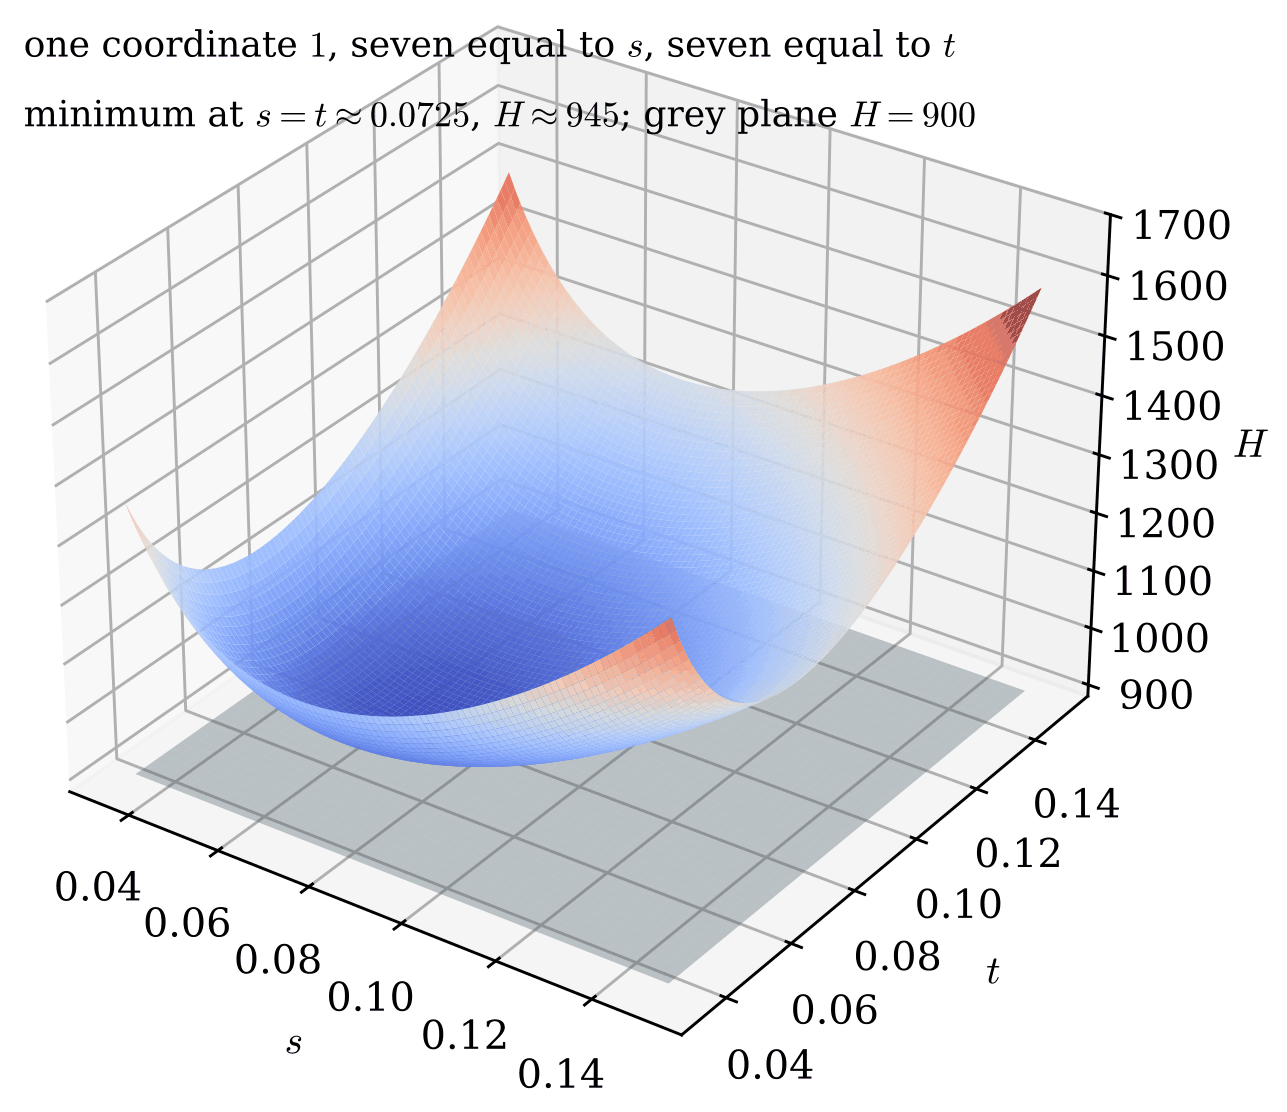
\includegraphics[width=\figw]{figures/fig_shape.png}
\caption{The function $H$ of Lemma~\ref{lem:shape} at $u=(1,s,\dots,s,
t,\dots,t)$ with seven coordinates $s$ and seven coordinates $t$. The
minimum is on the diagonal at $s=t=t_0\approx0.0725$, where $H\approx945$;
the grey plane is the level $900$ that the lemma needs.}
\label{fig:shape}
\end{figure}

\begin{proof}[Proof of Theorem~\ref{thm:bound}]
The cases $m\le14$ of the conjecture are theorems~\cite{All26} and the
references there. If two coordinates of a counterexample $v$ coincide, the
$15$ speeds take at most $14$ distinct values, and $\LRC(14)$ gives a time
with $\|tv_i\|\ge\frac1{15}>\frac1{16}$ for all $i$; so the coordinates are
pairwise distinct. If $2\le d\le16$ and no $v_i$ is divisible by $d$, then
$t=1/d$ gives $\|v_i/d\|\ge\frac1d\ge\frac1{16}$ for every $i$; so each
$d\le16$ divides some speed, and taking for $d$ the largest power of each
prime below $16$ shows that
$720720=\operatorname{lcm}(2,\dots,16)=2^4\cdot3^2\cdot5\cdot7\cdot11\cdot13$
divides the product~\cite[Lemma~4]{Ros26a}. Theorem~\ref{thm:flag} with
$n=15$, the ratio bound and Lemma~\ref{lem:shape} give
\[
 \log(v_1\cdots v_{15})\ <\ 15\log\frac{A_{15}}{30}\ =\ 497.02981257\ldots .
\]
If $\mathcal P$ is as in the statement, the pairwise coprime numbers
$720720$ and $p\in\mathcal P$ all divide $v_1\cdots v_{15}$, so
\begin{align*}
 \log(v_1\cdots v_{15})&\ \ge\ \log720720+\sum_{p\in\mathcal P}\log p\\
 &\ >\ 13.4880+483.5419\ =\ 497.0299 ,
\end{align*}
a contradiction.
\end{proof}

\section{Binary lifting at a power of two}\label{sec:binary}

For fourteen speeds the binary lifts stop at level $32$, and the residue
classes they leave are finished at level $15$, the first level whose time grid
contains $1/15$; the tuple $(1,\dots,14)$ is tight and survives every binary
level. For fifteen speeds the corresponding level is $16$, itself a power of
two, so the times $a/16$ are on the grid of the binary cascade from level
$16$ on, and the tight tuple $(1,\dots,15)$ is settled by the cascade
itself.\footnote{At $p=31$ the vector $(1,2,\dots,15)$ is the only level-one
class up to symmetry (Proposition~\ref{prop:small}), and all its lifts are
proper by level $16$; see Table~\ref{tab:small}.} What the factorisation
$15=3\cdot5$ did for fourteen speeds is done here by a shift lemma for powers
of two, and by lifting further.

\subsection{The shift lemma}

\begin{lemma}[Shift lemma]\label{lem:shift}
Let $K\ge3$, let $u_1,\dots,u_K$ be nonzero integers, and let $d=2^j$ with
$j\ge1$. Put $E=\{i:d\nmid u_i\}$ and, for $i\in E$, $g_i=\gcd(d,u_i)$ and
$N_i=d/g_i$. Assume $|E|\ge2$ and $\LRC(m)$ for every $m\le K-2$. If
\begin{equation}\label{eq:Sd}
 S_d\ =\ \sum_{i\in E}g_i\Bigl\lceil\frac{2N_i}{K+1}\Bigr\rceil\ <\ d,
\end{equation}
then there is a time $t$ with $\|tu_i\|\ge\frac1{K+1}$ for every $i$.
\end{lemma}

\begin{proof}
Let $B$ be the set of indices with $d\mid u_i$, so $|B|=K-|E|\le K-2$. The
absolute values of the integers $u_i/d$, $i\in B$, take $m\le K-2$ distinct
values, and $\LRC(m)$ gives $t_1$ with $\|t_1u_i/d\|\ge\frac1{m+1}\ge
\frac1{K+1}$ for $i\in B$ (if $B$ is empty take $t_1=0$). Put $t_0=t_1/d$
and consider the $d$ times $t_q=t_0+q/d$, $0\le q<d$. For $i\in B$,
$t_qu_i-t_0u_i=q(u_i/d)$ is an integer, so $\|t_qu_i\|\ge\frac1{K+1}$ for
every $q$.

Fix $i\in E$. As $q$ runs over $0,\dots,d-1$, the fractional part of
$qu_i/d$ runs over the grid $N_i^{-1}\Z/\Z$, hitting each point exactly
$g_i$ times. The shift $q$ is bad for $u_i$ when $t_0u_i+qu_i/d$ lies within
less than $\frac1{K+1}$ of an integer, that is, when $qu_i/d$ lies in a
fixed open arc of length $\frac2{K+1}<1$. An open arc of that length
contains at most $\lceil2N_i/(K+1)\rceil$ points of a grid of mesh $1/N_i$,
because an open interval of length $\ell$ contains at most $\lceil\ell\rceil$
integers. So $u_i$ forbids at most $g_i\lceil2N_i/(K+1)\rceil$ of the $d$
shifts, all exceptional speeds together forbid at most $S_d<d$ of them, and
some $t_q$ is a witness.
\end{proof}

For $d=2$ the sum is $S_2=|E|$, and the condition $S_2<2$ says that at most
one speed is odd: this is the gcd clause with the prime $2$. For an odd
prime $d$ the same argument is Allikvere's few-exception
shift~\cite[Lemma~4.6]{All26}, which adapts a shifting argument of
Rosenfeld~\cite[Lemma~5]{Ros26b}. Figure~\ref{fig:shift} shows the count for
$d=16$.\footnote{In the figure the exceptional speeds are congruent to
$1,3,2,4,6$ modulo $16$, with $g_i=1,1,2,4,2$; they forbid $2,2,2,4,2$ shifts,
at most the bounds $2,2,2,4,2$ of the lemma, $12$ in all, and four of the
sixteen shifts remain. The lemma itself needs only $S_{16}=12<16$ and does
not use the position of the bad arcs.}

\begin{figure}[t]
\centering
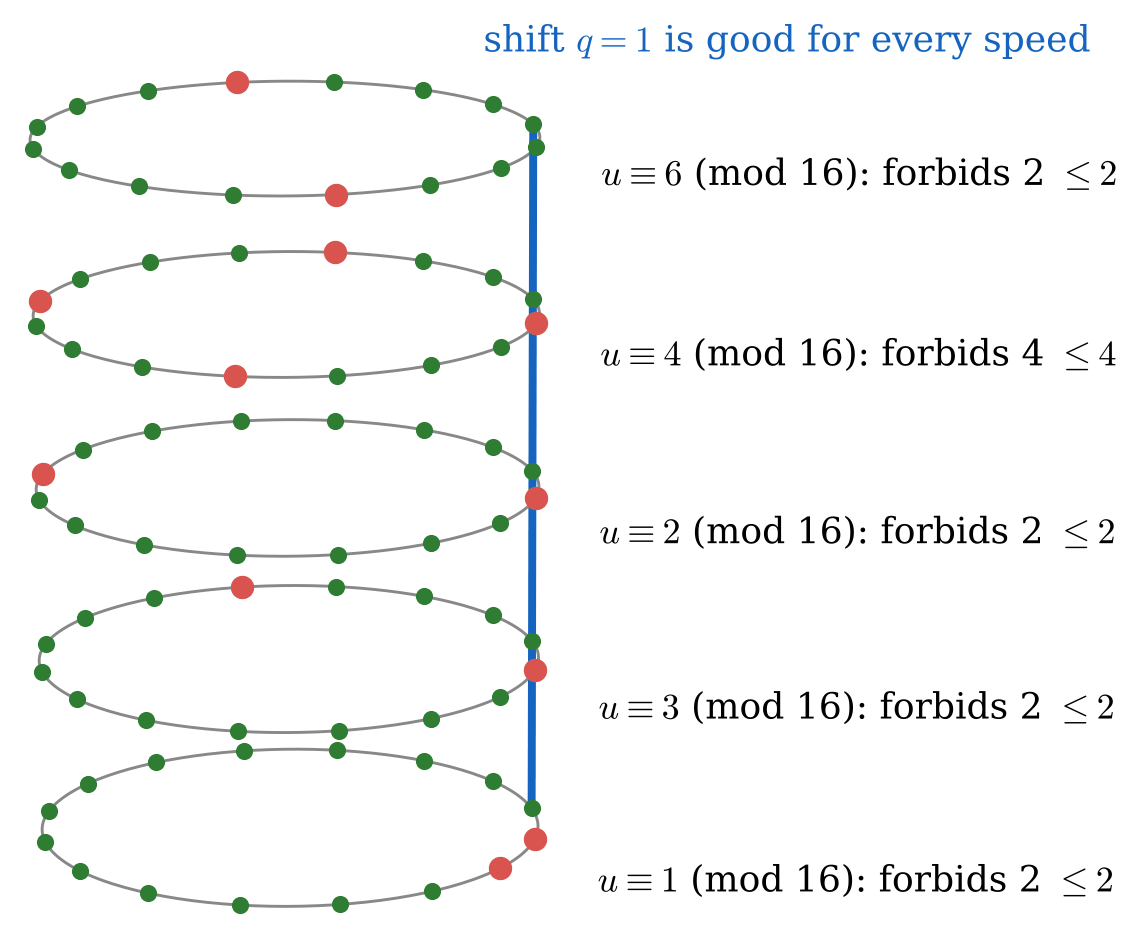
\includegraphics[width=\figw]{figures/fig_shift.png}
\caption{The shift lemma for $d=16$. Each ring is one exceptional speed;
its sixteen points are the shifts $q=0,\dots,15$, red where $t_0+q/16$ is
within $\frac1{16}$ of an integer multiple of $1/u_i$. The speeds divisible by
$16$ do not move. A shift that is green on every ring is a witness.}
\label{fig:shift}
\end{figure}

\begin{corollary}\label{cor:shiftclass}
Assume $\LRC(m)$ for every $m\le13$. Let $w\in\Z_{p,l}^{15}$ be improper at
level $l$, let $d=2^j$ divide $l$ with $j\ge2$, and suppose that the
coordinates of $w$ satisfy~\eqref{eq:Sd} with $K=15$, where $g_i$ is computed
from the residue of $w_i$ modulo $d$. Then every integer vector with nonzero
coordinates congruent to $w$ modulo $lp$ has the lonely-runner property, and
so does every integer vector with nonzero coordinates congruent to any lift
of $w$ to a higher level.
\end{corollary}

\begin{proof}
Since $d$ divides $lp$, an integer vector $x\equiv w\pmod{lp}$ has
$\gcd(d,x_i)=\gcd(d,w_i)$ for every $i$, so $x$ satisfies~\eqref{eq:Sd}.
Because $w$ fails the gcd clause, at least two coordinates are odd, hence
$|E|\ge2$. Lemma~\ref{lem:shift} with $K=15$ applies. A lift of $w$ to a
higher level is congruent to $w$ modulo $lp$, so the same holds for it.
\end{proof}

\subsection{Deeper lifting}

For a vector $u\in\Z_{p,1}^{15}$ the computation keeps the set of improper
lifts of $u$ at levels $2,4,8,\dots$ and removes at each level every lift to
which Corollary~\ref{cor:shiftclass} applies for some $d=2^j$ dividing the
level. If the set is empty at some level $l$, every lift of $u$ to level $l$
is proper, or descends from a lift that is proper at a lower level, or
descends from a lift removed by the corollary; by the persistence of
properness and Corollary~\ref{cor:shiftclass}, $u$ is settled at level $l$ in
the sense of Lemma~\ref{lem:symm}. Since the hypothesis of
Lemma~\ref{lem:criterion} only asks for some level, any depth may be used,
and the depth must be stated with the result.

The computation for fourteen speeds stopped at level $32$, and at first we
kept that depth. At the primes $19$, $23$, $37$ and $41$ it leaves classes
with improper lifts at level $32$. Each of these classes has several speeds
in one residue class modulo $p$, and each loses its last improper lifts at
level $64$ or $128$ (Table~\ref{tab:depth}). Repeated classes are expensive
because the coordinates in one class modulo $p$ differ only in their binary
digits, so the lifts that keep all of them close to the bad arcs of the
same times are many; the parity condition in the gcd clause cuts them down
only slowly. We therefore lift to level $128$, which settles every class met
at the primes of Table~\ref{tab:small}. At $p=23$ every one of the 91 orbit representatives keeps improper lifts at level $32$; they lose the last ones 57 at level $64$ and 34 at level $128$.

\begin{wtable}
\caption{Improper lifts of five level-one classes at the binary levels $16$
to $128$. A class is given by its speed residues; $1^7$ means seven speeds
congruent to $1$. The counts are of labelled lifts, after the gcd clause and
the shift lemma; a dash means that the class was already settled.}
\label{tab:depth}
\centering
\small
\begin{tabular}{@{}lllll@{}}
\toprule
$p$, class & $16$ & $32$ & $64$ & $128$\\
\midrule
$19$: $1^7,2,\dots,9$ & $3.98\cdot10^{9}$ & $1.18\cdot10^{10}$ & $2.14\cdot10^{10}$ & $0$\\
$23$: $1^5,2,\dots,11$ & $21{,}976{,}320$ & $593{,}280$ & $0$ & --\\
$23$: $1^3,2^2,3^2,4,\dots,11$ & $25{,}459{,}728$ & $3{,}335{,}616$ & $50{,}688$ & $0$\\
$37$: $1^7,3,4,7,9,10,11,12,16$ & $29{,}756{,}160$ & $82{,}615{,}680$ & $0$ & --\\
$41$: $1^6,3,4,7,10,11,12,13,16,18$ & $7{,}687{,}200$ & $11{,}865{,}600$ & $0$ & --\\
\bottomrule
\end{tabular}
\end{wtable}

\begin{figure}[t]
\centering
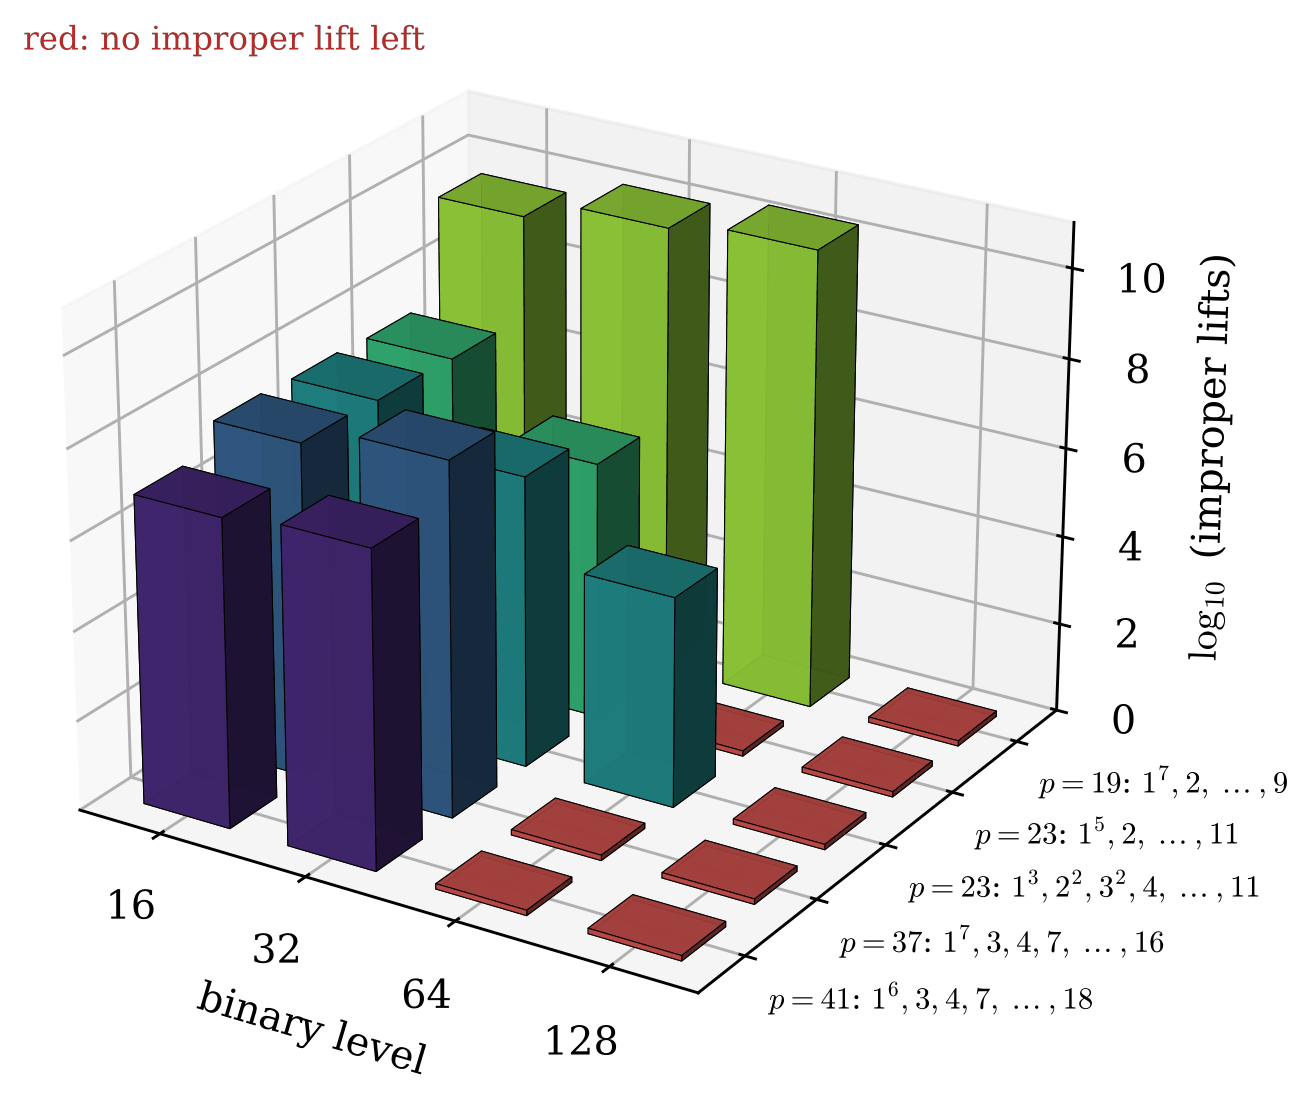
\includegraphics[width=\figw]{figures/fig_depth.png}
\caption{The counts of Table~\ref{tab:depth} on a logarithmic scale. Every
class still has improper lifts at level $32$, the depth used for fourteen
speeds, and none has any at level $128$.}
\label{fig:depth}
\end{figure}

The counts in Table~\ref{tab:depth} were computed twice, by the lifting
program and by an independent program that tests every time
$1,\dots,lp-1$ at every level from the definitions, with its own symmetry
reduction; they agree at every level.\footnote{Lifting a class with $r$
equal coordinates produces the same lifts up to the order of those
coordinates, so it suffices to expand, at each level, the lifts whose new
binary digits are non-decreasing along each group of equal coordinates,
each counted with the product of binomial coefficients $\binom{r}{s}$ that
gives the number of labelled lifts it represents. Both programs use this
reduction; they implement it independently, and the counts of labelled lifts
in Table~\ref{tab:depth} are exact integers.}

\section{The primes below thirty-two}\label{sec:small}

\begin{proposition}\label{prop:small}
Let $17\le p\le31$ be prime. A multiset of fifteen speed classes modulo $p$
is improper at level one if and only if it contains each of the
$\frac{p-1}2$ folded classes at least once.
\end{proposition}

\begin{proof}
By~\eqref{eq:cover}, a speed class $c$ covers a time class $a$ when
$16\,d_p(ac)<p<32$, that is, when $d_p(ac)=1$, which means $a\equiv\pm
c^{-1}\pmod p$. So each folded speed class covers exactly one folded time
class, and distinct speed classes cover distinct time classes. A multiset
covers all $\frac{p-1}2$ time classes exactly when it contains every speed
class.
\end{proof}

So for $p<32$ the level-one classes are the multisets formed by the
$\frac{p-1}2$ classes together with $15-\frac{p-1}2$ further classes chosen
freely, and there is no need for a covering search. We list all of them,
keep one representative of each orbit under permutations, sign changes and
units (Lemma~\ref{lem:symm}), and lift every representative to level $128$.
Table~\ref{tab:small} gives the numbers.

\begin{table}[t]
\caption{Level-one classes for the primes below $32$: the number of free
speeds, of multisets, and of orbits under permutations, sign changes and
units; the outcome of the lifting, and the number of lifts of the orbit
representatives settled by the shift lemma.}
\label{tab:small}
\centering
\small
\begin{tabular}{@{}rrrrll@{}}
\toprule
$p$ & free & multisets & orbits & outcome & shift lemma\\
\midrule
$23$ & $4$ & $1{,}001$ & $91$ & level $128$ & $8{,}636{,}800$\\
$29$ & $1$ & $14$ & $1$ & level $32$ & $0$\\
$31$ & $0$ & $1$ & $1$ & level $16$ & $0$\\
\bottomrule
\end{tabular}
\end{table}

\section{The larger primes}\label{sec:large}

From $p=37$ on, a speed class covers more than one time class and a
level-one class need not contain every speed class. We then follow the
two-branch search of~\cite[Sect.~4.1]{All26} with fifteen speeds. A
multiset that covers is either an irredundant cover on fifteen distinct
classes, or it contains a cover on at most fourteen classes, and the two
cases are searched separately. In the second case Allikvere's private-time
bound~\cite[Lemma~4.1]{All26}, which is stated for any number of speeds,
gives a class of multiplicity at most two with many times covered by it
alone; after removing one copy of a suitable class and moving that class to
$1$ by a unit, the search lists fourteen-class multisets satisfying the bound
and extends each by every class. The proof of completeness
of~\cite[Proposition~4.2]{All26} uses neither $k=13$ nor $k=14$ and gives,
for fifteen speeds, a representative of every orbit of improper level-one
vectors. When an exhaustive search shows that no cover uses at most thirteen
classes, every cover inside a fourteen-class support is minimal, and only
minimal fourteen-class covers need to be extended; otherwise all
fourteen-class multisets satisfying the bound are extended. Every class
found is then lifted as in Section~\ref{sec:binary}.

\begin{wtable}
\caption{The prime gates. For each prime the search variant, the number of
level-one vectors passed to the lifting (orbit representatives for the
primes below $32$), the level by which every lift is settled, the number of
lifts settled by the shift lemma, and the summed time of the jobs in hours
on a shared four-core machine. In the decomposition variant no cover uses
at most thirteen classes.}
\label{tab:results}
\centering
\small
\begin{tabular}{@{}rllrrr@{}}
\toprule
$p$ & variant & vectors & level & shift lemma & hours\\
\midrule
$23$ & small prime & $91$ & $128$ & $8{,}636{,}800$ & $1.9$\\
$29$ & small prime & $1$ & $32$ & $0$ & $<0.1$\\
$31$ & small prime & $1$ & $16$ & $0$ & $<0.1$\\
$179$ & general & $438{,}266{,}496$ & $16$ & $403{,}094{,}340$ & $9.9$\\
$239$ & decomposition & $10{,}536{,}820$ & $16$ & $0$ & $2.0$\\
$269$ & decomposition & $6{,}596{,}721$ & $16$ & $0$ & $5.1$\\
$271$ & decomposition & $4{,}179{,}959$ & $16$ & $0$ & $4.1$\\
$281$ & decomposition & $3{,}825{,}618$ & $16$ & $0$ & $7.5$\\
$283$ & decomposition & $2{,}821{,}058$ & $16$ & $0$ & $6.9$\\
\bottomrule
\end{tabular}
\end{wtable}

\begin{proof}[Proof of Theorem~\ref{thm:primes}]
For each $p\in\mathcal P_0$ the computation of Section~\ref{sec:small} or of
this section lists a representative of every orbit of improper level-one
vectors, and lifting leaves no improper lift at the level of
Table~\ref{tab:results}. By Lemma~\ref{lem:symm} every $u\in\Z_{p,1}^{15}$ is
settled at that level: if $u$ is proper at level one, all its lifts are
proper, and otherwise its orbit has a representative that the computation
settles. Lemma~\ref{lem:criterion}, whose hypothesis $\LRC(m)$ for $m<15$
is~\cite{All26} and the references there, gives $p\mid v_1\cdots v_{15}$ for
every primitive counterexample with distinct coordinates, and by
Theorem~\ref{thm:bound} the coordinates of every primitive counterexample are
distinct.
\end{proof}

The shift lemma is used in the proof: at $p=23$ it settles $8{,}636{,}800$ lifts; at $p=179$ it settles $403{,}094{,}340$ lifts, while at $29$, $31$, $239$, $269$, $271$, $281$ and $283$ no lift needs it. Without it these gates would leave improper lifts that no witness on the binary grid settles.

\section{What remains}\label{sec:remains}

By Theorem~\ref{thm:bound} the conjecture for sixteen runners follows from
prime gates whose logarithms add up to more than $483.5419$; the primes of
$\mathcal P_0$ give $43.0813$. One sufficient set is every prime from
$17$ to $523$, ninety-three primes; others trade small primes for large ones
(Fig.~\ref{fig:budget}). The work per prime is dominated by the covering
search. At $p=239$, where no cover uses at most thirteen classes, it took
about two hours on one core, about five times the corresponding cost for
fourteen speeds; at $p=179$, where such covers exist, the reducible branch
produced $2{,}676{,}385$ fourteen-class covers, each extended by all
$89$ classes, and the gate took about 10 hours. The time
grows with $p$ roughly like the number of irredundant covers, so the
complete set is a computation of thousands of core-hours with the programs
of this paper. The two smallest primes are not cheap either: at $p=19$ six
speeds are free, the lift tree of a single orbit grows about fourfold with
each doubling of the level, and one orbit can take hours. Nothing in the
method fails at the primes we have run: every class met so far is settled
by level $128$.

\begin{figure}[t]
\centering
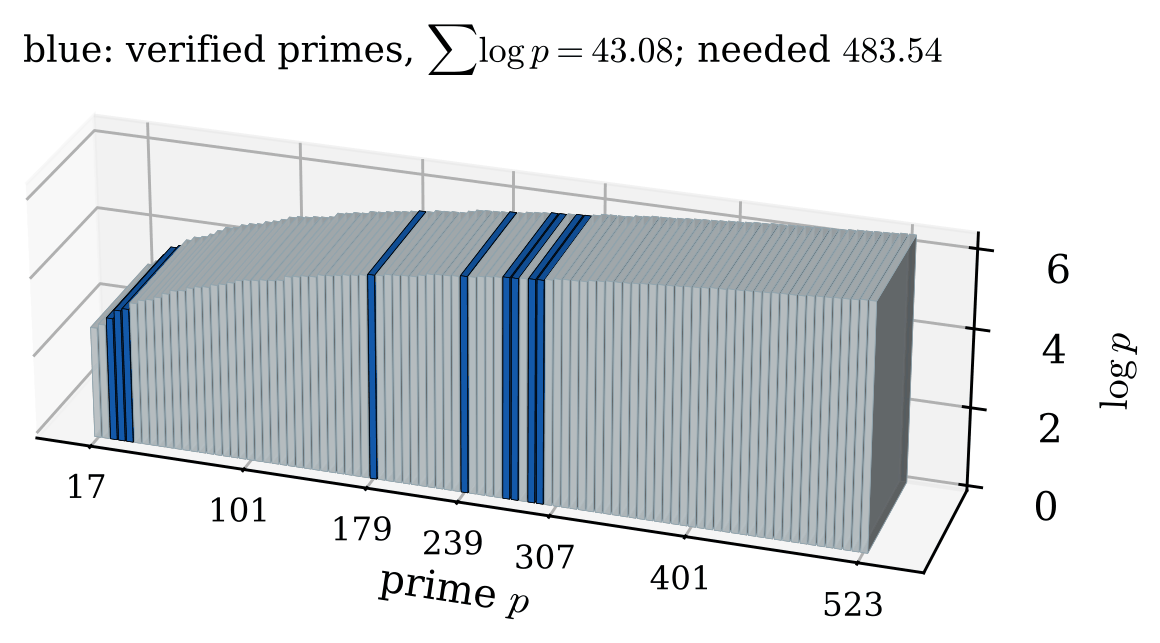
\includegraphics[width=\figw]{figures/fig_budget.png}
\caption{The logarithms of the primes from $17$ to $523$, whose sum exceeds
the $483.54$ that Theorem~\ref{thm:bound} requires. The primes of
Theorem~\ref{thm:primes} are marked.}
\label{fig:budget}
\end{figure}

The computations followed the learn-from-failure protocol of Anaxia, the
BLLM engine~\cite{Ana26,BB26c}.\footnote{The protocol records each attempt
that fails with its diagnosis, the rule it changed and the outcome of the
retry, and later attempts are checked against the rules; release~3.1.0 holds
the records of this work. Anaxia produced none of the constructions,
lemmas or computations of this paper. Two rules entered its log from this
work. Survivors of a search that stops at a fixed depth are not obstructions
when the property being tested is monotone in the depth, so the search must
be run deeper, with the depth stated in every result; the classes of
Table~\ref{tab:depth} were first taken for obstructions at level $32$. And
when an exact computation outgrows the hardware, the engine's skill memory,
rebuilt from its log, ranks a reduction, a larger budget and a new order of
the work as the changes that have helped before; this paper uses the third,
running the primes in order of measured cost per unit of log-sum, which
leaves the gates at $17$ and $19$ for later.}

\section*{Data and code availability}

Lemmas~\ref{lem:criterion}, \ref{lem:symm}, \ref{lem:shape}
and~\ref{lem:shift}, Corollary~\ref{cor:shiftclass},
Proposition~\ref{prop:small} and Theorem~\ref{thm:bound} are proved by
hand; the numerical steps of Lemma~\ref{lem:shape} are in
Appendix~\ref{app:shape}. Theorem~\ref{thm:primes} rests on the computation
described in Sections~\ref{sec:binary} to~\ref{sec:large}. The repository
\texttt{creelie/Math-repo1} contains the \LaTeX{} source of this paper; the
cover generator and the lifting program, adapted from Allikvere's
code~\cite{All26code}, with a notice of every change; the scripts that run
the prime gates; the summary and the SHA-256 manifest of every gate in
Table~\ref{tab:results}; the independent lifting program that tests every
time from the definitions; the exact checks of the shape bound, of the
constants of Table~\ref{tab:cr} and of the shift lemma; and the measured
costs. The archive is~\cite{Archive}, \archivelink, where later versions are
listed. The search followed the learn-from-failure protocol of the BLLM
engine Anaxia, release~3.1.0~\cite{Ana26}, described in~\cite{BB26c}. Deep
Bhattacharjee carried out the computations and the C++, Python and shell
checks with AI assistance from Claude (Anthropic); both authors approved the
final text.

\section*{Ethical declarations}

\emph{Funding.} None. \emph{Competing interests.} None.


\appendix

\section{The constants and the numerical steps of the shape bound}\label{app:shape}

\subsection{The constants of the flag bound}

For $n=15$ we have $B_r=\bigl(r/(8(16-r))\bigr)^2$. Table~\ref{tab:cr} lists
$c_r=B_r-B_{r-1}$ and the ratios $c_{r+1}/c_r$. All entries are exact. The
product of the fourteen values $c_r$ is the constant $K_{15}$ of
Section~\ref{sec:shape}, and
\begin{align*}
 15\log\frac{A_{15}}{30}&=-\frac{15}2\log K_{15}-15\log30\\
 &=497.0298125704945\ldots ,
\end{align*}
computed with fifty significant digits. Since
\[
 \log720720=13.4880059913253\ldots ,
\]
the logarithms of the primes $p\ge17$ must add up to more than
\[
 483.5418065791692\ldots .
\]

\begin{table}[t]
\caption{The increments $c_r=B_r-B_{r-1}$ of the prefix bounds for fifteen
speeds and their ratios. The least ratio is at $r=6$.}
\label{tab:cr}
\centering
\small
\begin{tabular}{@{}rlll@{}}
\toprule
$r$ & $c_r$ & $c_{r+1}/c_r$ & \\
\midrule
$1$ & $1/14400$ & $176/49$ & $3.5918$\\
$2$ & $11/44100$ & $3825/1859$ & $2.0576$\\
$3$ & $17/33124$ & $539/306$ & $1.7614$\\
$4$ & $11/12168$ & $2197/1331$ & $1.6506$\\
$5$ & $13/8712$ & $522/325$ & $1.6062$\\
$6$ & $29/12100$ & $3751/2349$ & $1.5968$\\
$7$ & $31/8100$ & $50/31$ & $1.6129$\\
$8$ & $1/162$ & $81/49$ & $1.6531$\\
$9$ & $1/98$ & $31/18$ & $1.7222$\\
$10$ & $31/1764$ & $1421/775$ & $1.8335$\\
$11$ & $29/900$ & $117/58$ & $2.0172$\\
$12$ & $13/200$ & $275/117$ & $2.3504$\\
$13$ & $11/72$ & $34/11$ & $3.0909$\\
$14$ & $17/36$ &  & \\
\bottomrule
\end{tabular}
\end{table}

\subsection{The inequalities in the proof of Lemma~\ref{lem:shape}}

Every inequality below compares two rational numbers, after raising both
sides to a power that clears the fractional exponents; the decimal values
are given to show the margins.

\emph{The root $\alpha$.} The polynomial $g(u)=14u^2-13u+1$ takes the
values
\begin{gather*}
 g(0.0846)=0.00040024>0,\\
 g(0.0847)=-0.00066274<0,
\end{gather*}
so the smaller root $\alpha$ of $g$ lies in $(0.0846,0.0847)$.

\emph{The sign of $P$.} For $0<u<\alpha<0.0847$ the terms $7u^5+14u^4$ are
positive and $-4u-11u^2-27u^3$ is decreasing, so
\begin{align*}
 P(u)&>1-4(0.0847)-11(0.0847)^2-27(0.0847)^3\\
 &=0.565878\ldots>0 .
\end{align*}

\emph{The lower bound for $a(\alpha)$.} Since $q$ increases on $(0,1)$ and
$u^{-2/15}$ decreases, $a(\alpha)>q(0.0846)/0.0847^{2/15}$. Raising to the
fifteenth power, the claim $q(0.0846)/0.0847^{2/15}>\frac85$ becomes
\begin{align*}
 q(0.0846)^{15}&=9.51331\ldots\\
 &>\Bigl(\frac85\Bigr)^{15}(0.0847)^2=8.27116\ldots .
\end{align*}

\emph{Two or more coordinates equal to one.} The ratio of consecutive
values of $f(k)=\frac k2\,2^k\bigl(\frac85\bigr)^{15-k}$ is
$f(k+1)/f(k)=\frac{k+1}k\cdot\frac54>1$, so $f$ increases, and
$f(2)=4\bigl(\frac85\bigr)^{13}=1801.43\ldots$.

\emph{The root $t_0$.} The cubic $378t^3+25t^2+10t-1$ takes the values
$-0.0015037\ldots$ at $t=0.0724$ and $0.00045378\ldots$ at $t=0.0725$.

\emph{The value $H(t_0)$.} The factors $1+2t+27t^2$ and $q(t)$ increase
and $t^{-28/15}$ decreases, so on $[0.0724,0.0725]$
\[
 H(t)\ \ge\ \frac{(1+2\cdot0.0724+27\cdot0.0724^2)\,q(0.0724)^{13}}
 {0.0725^{28/15}} .
\]
Raising to the fifteenth power, the right side exceeds $942.5$ because
\begin{align*}
 (1+2\cdot0.0724&+27\cdot0.0724^2)^{15}\,q(0.0724)^{195}\\
 &=5.05703\ldots\cdot10^{12},\\
 942.5^{15}\cdot0.0725^{28}&=5.05457\ldots\cdot10^{12}.
\end{align*}
The bound itself is $942.53\ldots$, against the true minimum
$H(t_0)=944.96\ldots$ at $t_0=0.0724768\ldots$.

\emph{The extremal shape.} The minimum of $H$ is attained at the point
$u=(1,t_0,\dots,t_0)$, where
\[
 R_{15}=\bigl(225/H(t_0)\bigr)^{1/2}=0.48796\ldots .
\]
Using $\frac12$ in place of this value in Theorem~\ref{thm:flag} weakens
the logarithmic bound by $15\log(0.5/0.48796)=0.366$.

\subsection{The algebraic identities}

The identities used in the proof are checked by expanding both sides as
rational functions: the formula~\eqref{eq:phiprime} for $\varphi'$, the
identity $14q(u)+g(u)=15(1+u)$, the formula for $L'$, the logarithmic
derivative of $a$, the closed form of $H(t)$ on the line
$u=(1,t,\dots,t)$ and its logarithmic derivative. For the last one,
\[
 \frac{d}{dt}\log H(t)=\frac{2+54t}{1+2t+27t^2}+\frac{13(2-2t)}{q(t)}
 -\frac{28}{15t},
\]
and putting the three terms over the common denominator
$15t\,q(t)(1+2t+27t^2)$ gives the numerator
$-28(t-1)(378t^3+25t^2+10t-1)$; since $q(t)=-(t^2-2t-1)$, this is the
expression in the proof.

\begin{thebibliography}{99}\raggedright\advance\leftskip\labelwidth

\bibitem{All26}
J.~Allikvere, Fourteen and fifteen lonely runners, preprint (2026),
\href{https://arxiv.org/abs/2609.02604v2}{arXiv:2609.02604v2}.

\bibitem{All26code}
J.~Allikvere, Fifteen lonely runners: manuscript, gate certificates, and
audit code, Zenodo (2026),
\href{https://doi.org/10.5281/zenodo.22667683}{doi:10.5281/zenodo.22667683}.

\bibitem{BS08}
J.~Barajas and O.~Serra, The lonely runner with seven runners, Electron. J.
Combin. \textbf{15} (2008), Paper No.~R48,
\href{https://doi.org/10.37236/772}{doi:10.37236/772}.

\bibitem{BB26c}
D.~Bhattacharjee and U.~Bhattacharya, BLLM: Beyond the LLM with Deep
Human-Mind-AI, preprint (2026), distributed with~\cite{Ana26}.

\bibitem{Ana26}
D.~Bhattacharjee, Anaxia, the BLLM engine, eBLLM release 3.1.0, Zenodo
(2026), \href{https://doi.org/10.5281/zenodo.23484160}{doi:10.5281/zenodo.23484160};
all versions
\href{https://doi.org/10.5281/zenodo.23286641}{doi:10.5281/zenodo.23286641}.

\bibitem{BBB26a}
D.~Bhattacharjee, U.~Bhattacharya and S.~Bhattacharya, The sphere packing
problem in dimension 4, Preprints (2026),
\href{https://doi.org/10.20944/preprints202606.0856.v11}{doi:10.20944/preprints202606.0856.v11}.

\bibitem{BBB26b}
D.~Bhattacharjee, U.~Bhattacharya and S.~Bhattacharya, The sphere packing
problem in dimension 7, Preprints (2026),
\href{https://doi.org/10.20944/preprints202606.1534.v9}{doi:10.20944/preprints202606.1534.v9}.

\bibitem{BGGST98}
W.~Bienia, L.~Goddyn, P.~Gvozdjak, A.~Seb\H{o} and M.~Tarsi, Flows, view
obstructions, and the lonely runner, J. Combin. Theory Ser.~B \textbf{72}
(1998), 1--9,
\href{https://doi.org/10.1006/jctb.1997.1770}{doi:10.1006/jctb.1997.1770}.

\bibitem{BCS26}
M.~Blanco, F.~Criado and F.~Santos, Coloopless zonotopes and
counterexamples to the Shifted Lonely Runner Conjecture, preprint (2026),
\href{https://arxiv.org/abs/2603.24784}{arXiv:2603.24784}.

\bibitem{BHK01}
T.~Bohman, R.~Holzman and D.~Kleitman, Six lonely runners, Electron. J.
Combin. \textbf{8} (2001), Paper No.~R3,
\href{https://doi.org/10.37236/1602}{doi:10.37236/1602}.

\bibitem{Cus73}
T.~W. Cusick, View-obstruction problems, Aequationes Math. \textbf{9}
(1973), 165--170,
\href{https://doi.org/10.1007/BF01832623}{doi:10.1007/BF01832623}.

\bibitem{CP84}
T.~W. Cusick and C.~Pomerance, View-obstruction problems, III, J. Number
Theory \textbf{19} (1984), 131--139,
\href{https://doi.org/10.1016/0022-314X(84)90097-0}{doi:10.1016/0022-314X(84)90097-0}.

\bibitem{GK26}
V.~Giri and N.~Kravitz, The structure of Lonely Runner spectra, Math. Proc.
Cambridge Philos. Soc. \textbf{180} (2026), 343--361,
\href{https://doi.org/10.1017/S0305004125101497}{doi:10.1017/S0305004125101497}.

\bibitem{GW06}
L.~Goddyn and E.~B. Wong, Tight instances of the lonely runner, Integers
\textbf{6} (2006), Paper No.~A38.

\bibitem{KZ1873}
A.~Korkine and G.~Zolotareff, Sur les formes quadratiques, Math. Ann.
\textbf{6} (1873), 366--389,
\href{https://doi.org/10.1007/BF01442795}{doi:10.1007/BF01442795}.

\bibitem{LLS90}
J.~C. Lagarias, H.~W. Lenstra, Jr. and C.~P. Schnorr, Korkin--Zolotarev
bases and successive minima of a lattice and its reciprocal lattice,
Combinatorica \textbf{10} (1990), 333--348,
\href{https://doi.org/10.1007/BF02128669}{doi:10.1007/BF02128669}.

\bibitem{MSS25}
R.~D. Malikiosis, F.~Santos and M.~Schymura, Linearly exponential checking
is enough for the lonely runner conjecture and some of its variants, Forum
Math. Sigma \textbf{13} (2025), Paper No.~e164,
\href{https://doi.org/10.1017/fms.2025.10107}{doi:10.1017/fms.2025.10107}.

\bibitem{PS24}
G.~Perarnau and O.~Serra, The Lonely Runner Conjecture turns 60, preprint
(2024), \href{https://arxiv.org/abs/2409.20160}{arXiv:2409.20160}.

\bibitem{Ros26a}
M.~Rosenfeld, The lonely runner conjecture holds for eight runners, Math.
Comp. (2026), \href{https://doi.org/10.1090/mcom/4243}{doi:10.1090/mcom/4243}.

\bibitem{Ros26b}
M.~Rosenfeld, The lonely runner conjecture holds for nine runners, preprint
(2026), \href{https://arxiv.org/abs/2512.01912}{arXiv:2512.01912}.

\bibitem{ST26}
T.~Sungkawichai and T.~Trakulthongchai, Eleven, twelve, and thirteen lonely
runners, preprint (2026),
\href{https://arxiv.org/abs/2604.23906}{arXiv:2604.23906}.

\bibitem{Tao18}
T.~Tao, Some remarks on the lonely runner conjecture, Contrib. Discrete
Math. \textbf{13} (2018), no.~2,
\href{https://doi.org/10.55016/ojs/cdm.v13i2.62728}{doi:10.55016/ojs/cdm.v13i2.62728}.

\bibitem{Tra26}
T.~Trakulthongchai, Nine and ten lonely runners, Electron. J. Combin.
\textbf{33} (2026), no.~2, Paper No.~P2.46,
\href{https://doi.org/10.37236/14972}{doi:10.37236/14972}.

\bibitem{Wil67}
J.~M. Wills, Zwei S\"atze \"uber inhomogene diophantische Approximation von
Irrationalzahlen, Monatsh. Math. \textbf{71} (1967), 263--269,
\href{https://doi.org/10.1007/BF01298332}{doi:10.1007/BF01298332}.

\bibitem{Archive}
D.~Bhattacharjee and U.~Bhattacharya, Sixteen lonely runners: prime gates,
source and certificates, \ifx\zenodoID\empty GitHub repository
\texttt{creelie/Math-repo1}\else Zenodo\fi{} (2026), \archivelink.

\end{thebibliography}

\end{document}
